%%%%%%%%%%%%%%%%%%%%%%%%%%%%%%%%%%%%%%%%%%%%%%%%%%%%%%%%%%%%%%%%%%%%%%%%%%%%%%%%
%%
%%   BornAgain User Manual
%%
%%   homepage:   http://www.bornagainproject.org
%%
%%   copyright:  Forschungszentrum Jülich GmbH 2016
%%
%%   license:    Creative Commons CC-BY-SA
%%
%%   authors:    Scientific Computing Group at MLZ Garching
%%               M. Ganeva, G. Pospelov, W. Van Herck, J. Wuttke
%%
%%%%%%%%%%%%%%%%%%%%%%%%%%%%%%%%%%%%%%%%%%%%%%%%%%%%%%%%%%%%%%%%%%%%%%%%%%%%%%%%

\newpage
\chapter{The three interfaces of \BornAgain}  \label{sec:API3}

\section{Architectural overview}

The overall architecture of \BornAgain\ is outlined in \cref{Farch1}.
The core of \BornAgain\
\index{Core|see {\Code{libBornAgainCore}}}
comprises functionality to construct arbitrary hierarchical sample models,
to setup instrument models,
and to compute the expected detector image for any given sample and instrument model.
Furthermore \BornAgain\ comes with various minimizers that optimize model parameters
to fit the simulated detector image to a given experimental image.
All this functionality is implemented in a library, \Code{libBornAgainCore}.

\begin{figure}[tbh]
\begin{center}
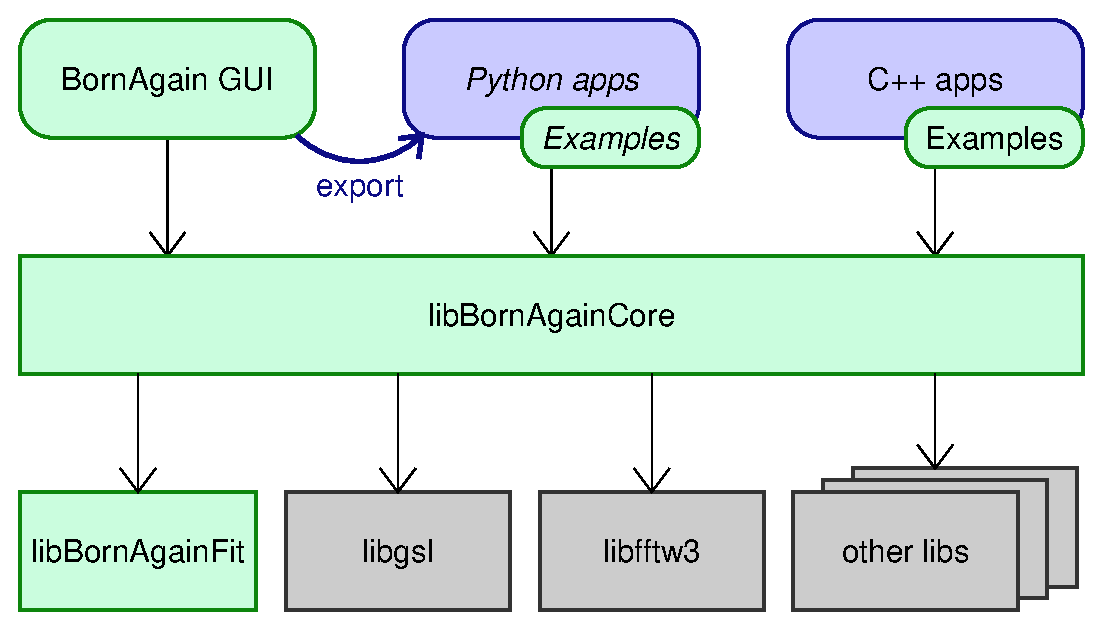
\includegraphics[width=0.8\textwidth]{fig/drawing/architecture1.ps}
\end{center}
\caption{Overall architecture of \BornAgain.
\index{Architecture!applications and libraries}%
Applications are shown as oval fields, libraries as rectangles.
Green fields designate software that is part of \BornAgain.
Gray fields are external dependences
(only two external libraries are explicitly shown;
several more are listed in the online compilation instructions).
Blue fields indicate stand-alone applications that use \BornAgain's
two Application Programming Interfaces (the C$++$ API and the Python API).
\index{C++!using BornAgain from}
\index{Python!using BornAgain from}
\index{Application Programming Interface}
While such applications are to be written by users,
some examples come with the \BornAgain\ source distribution,
and are explained in the following Manual chapters.
It is also possible to export a simulation setup from GUI as Python code.}
\label{Farch1}
\end{figure}

\index{libBornAgainCore@\Code{libBornAgainCore}}
This library, in turn, depends on a number of other libraries.
One of these, the minimizer wrapper \Code{libBornAgainFit}
\index{libBornAgainFit@\Code{libBornAgainFit}}
\index{Minimizers|see \Code{libBornAgainFit}}
has been written specifically for use in \BornAgain,
and for the time being is only distributed as part of \BornAgain,
though in the future it may find applications in other contexts.
The other library dependences of \Code{libBornAgainCore}
are multi-purpose libraries that are easily available as open-source packages.
\index{Dependences!libraries}

The library \Code{libBornAgainCore} can be used in three different ways:
From its graphical user interface (GUI), or
from user-written stand-alone applications in the programming languages C$++$ or Python.
These different approaches are briefly outlined below.
The Python interface is then described at length in the next chapters.

\section{Using BornAgain from its Graphical User Interface}
\index{Graphical User Interface|(}
\index{bornagain@\Code{bornagain}|see {Graphical User Interface}}
\index{Graphical User Interface|)}

\section{Using BornAgain from application programs}
\index{C++!using BornAgain from|(}
\index{Python!using BornAgain from|(}

The library \Code{libBornAgainCore}
\index{libBornAgainCore@\Code{libBornAgainCore}}%
\index{C++!libBornAgainCore@{\Code{libBornAgainCore} written in}}%
is written in the programming languages C++,
and therefore natively supports usage from application programs written in C++.


\index{C++!using BornAgain from|)}
\index{Python!using BornAgain from|)}
